%\documentclass{article}
\documentclass[a4paper, fleqn]{template/cas-dc}
\usepackage{template/cas-common}
\usepackage[numbers]{natbib}
\usepackage{geometry}
\usepackage{fleqn}

\usepackage{graphicx}
\usepackage{subcaption}
\usepackage{amsmath}
\usepackage{amsfonts}
\usepackage{amssymb}
\usepackage{comment}
%\usepackage{todonotes}
\usepackage{float}
% Math operators
\newcommand{\opt}{^*}
\newcommand{\voidarg}{{\,\cdot\,}}
\newcommand{\E}[2]{\operatorname{\mathbb{E}}_{#1}\left[#2\right]}
\newcommand{\density}{p}
\newcommand{\ent}{\mathcal{H}}
\newcommand{\Rset}{\mathbb R}

% MDP
\newcommand{\sspace}{\mathcal{S}}
\newcommand{\aspace}{\mathcal{A}}
\newcommand{\state}{\mathbf{s}}
\newcommand{\action}{\mathbf{a}}

\newcommand{\at}{{\action_t}}
\newcommand{\atp}{{\action_{t+1}}}
\newcommand{\st}{{\state_t}}
\newcommand{\stp}{{\state_{t+1}}}
\newcommand{\pdyn}{\density}

% reward
\newcommand{\reward}{r}
\newcommand{\rmin}{r_\mathrm{min}}
\newcommand{\rmax}{r_\mathrm{max}}

% Value and Q function
\newcommand{\Q}{Q}

% policy
\newcommand{\policy}{\pi}
\newcommand{\pparams}{{\phi}}   % policy parameters
\newcommand{\params}{\theta}

%  kernel
\newcommand{\discount}{\gamma}

\title[mode=title]{An explorational test method for learning vehicle control system robustness against sensor noise and false data injection attack}
\date{2025-08-27}
\author{Gábor Lóránt}

\begin{document}
	\begin{keywords}
		fuzz testing \sep deep reinforcement learning \sep functional safety \sep cyber security \sep automotive
	\end{keywords}
	
	
	\maketitle
	
	\begin{abstract}
		Fuzz testing (or fuzzing) is a dynamic software testing technique that involves sending random, malformed, or unexpected inputs to a system to uncover vulnerabilities, crashes, or unexpected behavior. In automotive systems, this is particularly useful for testing Electronic Control Units (ECUs), in-vehicle communication protocols (e.g., CAN, LIN, FlexRay) or diagnostic interfaces (e.g., UDS - ISO 14229). A custom fuzzer can be used to target the CAN bus and simulate attacks or faults, helping engineers identify weaknesses before vehicles go into production. The implementation of fuzz testing can be challenging in terms of efficiency in finding issues in the vehicle or its components. 
		The proposed test method explores the stability of the investigated control system, the quality of its sensor signal conditioning algorithms and its ability to learn external interventions. The proposed method automatically find the worst controller performance by keeping its base operation alive. The optimized test schedule and can be repetitively used later to evaluate the control algorithm as well as its infrastructure like signal conditioning and security protection.
	\end{abstract}
	
	\section{Introduction}
	
	ISO 26262 (international standard for functional safety in road vehicles, focusing on electrical/electronic systems) primarily addresses systematic failures and random hardware faults, fuzz testing complements it by targeting software robustness—especially in scenarios involving unexpected or malformed inputs. This is particularly relevant for advanced driver assistance systems (ADAS), autonomous driving features and vehicle communication protocols (e.g., CAN, LIN, Ethernet). Fuzz testing can be integrated into the verification and validation phases of ISO 26262 to uncover hidden software vulnerabilities that might compromise safety.
	
	While ISO/SAE 21434 standard governs cybersecurity engineering for road vehicles. It explicitly recommends fuzz testing as part of the validation process. Components rated CAL (Cybersecurity Assurance Level) 2 or higher should undergo fuzz testing. CAL 3 and 4 require advanced fuzzing, including adaptive input generation. Fuzz testing shall be applied early and systematically throughout the product lifecycle to detect vulnerabilities and reduce remediation costs. Furthermore fuzzing supports TARA (Threat Agent Risk Assessment) by automating risk identification and mitigation.
	
	Modern vehicles rely on numerous Electronic Control Units (ECUs) that communicate via the Controller Area Network (CAN) to manage critical functions efficiently. While the CAN enables efficient vehicle control through inter-ECU communication, it presents critical security vulnerabilities. Notably, the broadcast nature of CAN messages, transmitted without encryption, allows adversaries to eavesdrop on all network traffic. Additionally, the absence of access control and authentication mechanisms permits attackers to inject malicious messages, potentially compromising vehicle safety and control.
		
	\subsection{Related work}
	
	The integration of advanced cybersecurity mechanisms has significantly increased the complexity of testing processes, particularly within simulation environments and during test execution  \cite{marksteiner2021using}. While several testing methodologies have been proposed, many have only been validated in limited-scale configurations involving a small number of ECUs \cite{oruganti2019hardware}. Moreover, a notable gap persists in the development of robust and standardized metrics for evaluating fuzz testing effectiveness \cite{fowler2019method}.
	
	Cybersecurity testing in the automotive domain often prioritizes automated test case generation to satisfy predefined requirements. However, penetration testing remains predominantly manual, and the adaptation of fuzz testing techniques from traditional IT systems to automotive contexts presents opportunities for enhancement—particularly in terms of improving testing efficiency and scalability.
	
	A security analysis and reverse engineering case study conducted on an instrument cluster ECU demonstrated the applicability of fuzz testing during the later stages of product development \cite{anistoroaei2022security}. Future research should aim to enhance the methodologies for extracting meaningful and actionable metrics from fuzz testing processes.
	
	Furthermore, a recent study \cite{wang2020real} have proposed sensor-based solutions for automotive systems that concurrently enhance safety—by meeting real-time and recovery requirements—and cybersecurity, through improved attack detection capabilities. The existing security models are not enough robust yet because the busload of CAN and level of cryptographic strategy are not considered enough to be implemented in the frame. The enhancement of CAN, which has been upgraded to Controller Area Network with Flexible Data Rate (CAN-FD), provides high bandwidth and bigger payload, is a basis of new security models based on encryption and authentication.\cite{AUTOSAR_SecOC_R24_11}
	
	Fuzz testing techniques have evolved since its introduction, American Fuzzy Lop (AFL) is a fuzz testing framework that utilizes an instrumentation method and a genetic algorithms to generate diverse test cases, enabling the discovery of numerous software vulnerabilities \cite{zalewski2017american}. Despite its widespread adoption and proven effectiveness, AFL relies on blind mutation strategies lacking guided input generation. To overcome these limitations, several improved variants have been developed, including AFLFast \cite{bohme2016coverage}, AFL++ \cite{fioraldi2020afl++} and fuzzing based on Control Flow Graph Optimization \cite{10662925}. To improve the possibility of exposing defects, fuzzers use feedback from executions, such as execution state, results and fitness. A typical fitness is base on code coverage, which is used to determine the reward for the generated inputs. The current fuzzers have a common improvement of optimizing fuzzing process or enrich the information for fitness by utilizing among others machine learning and deep learning methods.\cite{zhu2022fuzzing}
	
	Automotive security testing primarily targets the vehicle's attack surfaces, which are typically located on either external communication interfaces (e.g., Vehicle-to-Everything, V2X) or internal network systems (e.g., In-Vehicle Networks, IVN). Machine learning classifiers are used to generate a risk score associated with the failure class, relative severity, and robustness of the failure from the vast fuzzing logs \cite{kayas2023ai}. 
	For testing intrusion detection algorithms a fuzzer generating messages conform to the in-vehicle communication protocol by utilizing Generative Adversarial Networks (GAN) was developed \cite{li2022gan}.
	
	Deep Reinforcement Learning (DRL) methods proposed widely to address cyberattacks including DRL-based security methods for cyber–physical systems, autonomous intrusion detection techniques, and multiagent DRL-based game theory simulations for defense strategies \cite{nguyen2021deep} \cite{ferdowsi2018robust}.
	
	\subsection{Motivation and ambitions}
	
	One of the widespread technique used by attackers is the masquerade attack. The attack manipulates the normal communication flow to a targeted ECU by injecting forged messages into the CAN network, thereby disrupting legitimate message delivery. This scenario presents significant challenges for simulation, as it necessitates the compromise of one or more components in the vehicle network (ECUs or sensors). Accurately replicating such conditions would require programming the simulated component to exhibit vulnerabilities analogous to those found in real-world systems, which extends beyond the scope of CAN bus simulation and is highly dependent on the specific characteristics of the individual ECUs. As a result, this type of attack lacks generalization across different CAN bus implementations.
	
	The fuzzing procedure consists of injecting CAN messages with both randomized identifiers and messages with valid CAN identifiers but randomized payloads, in order to systematically evaluate the response behavior of Electronic Control Units (ECUs) within the network. This capability is particularly advantageous when actual vehicle components are integrated into a testbed, as it enables researchers to monitor their responses to a range of CAN messages. Such observations may reveal unwanted functionalities or latent vulnerabilities within the system. 
	
	To identify CAN messages capable of influencing safety-critical ECU operations, researchers have explored CAN fuzzing techniques. However, existing approaches typically generate fuzzing inputs randomly without accounting for message content, leading to prolonged fuzzing duration.
	
	The main focus of existing fuzzing solutions to test the vehicle communication network, its intrusion detection capabilities and gateway securities \cite{9713864},\cite{8416255}, \cite{9719242}, \cite{fowler2019method}.
				
	This paper outlines a concept of an automated black-box test environment for verification of ECU behavior on masquerade attack as well as sensitivity of noise present in the vehicle network. The concept can be developed to a test framework for evaluation functional safety and cyber security requirements.
	
	\section{Methodology}
	\subsection{Smart fuzz test tool for vehicle control}
	
	The proposed test method operates in a digitally controlled closed loop system, like a modern vehicle. The vehicle dynamics control can be described model implements controllers for engine control units (ECUs), transmissions and anti-lock braking systems (ABS). The vehicle under control can be described as a coninuous-time system.
	
	\begin{equation}					
		\begin{aligned}
			\dot{x}(t) = f(x(t),u(t)) \\				
			y(t) = h(x(t),u(t))
		\end{aligned}	
	\end{equation}
	
	with the state $x(t)\in\Rset^n$, the control input $u(t)\in\Rset^m$, the output $y(t)\in\Rset^p$, $f$ describe the system dynamics and $h$ the output. The controller task is to maximize the output $y(t)$. The vehicle is controlled with ECUs that produce a discrete-time input $u[k]$ from a sampled state $x[k]$. See Figure~\ref{fig:system1}. Here, $x[k]$ is the state $x(t)$ sampled at $t = k\Delta t$, $k=0, 1, \ldots$, for some sampling period $\Delta t > 0$ and $u[k]$ is converted to the continuous-time input $u(t)$ by $u(t) = u[k]$ for $k \Delta t\leq t<(k+1)\Delta t$ and $k=0, 1, \ldots$.				
	
	\begin{figure}[h]
		\begin{center}
			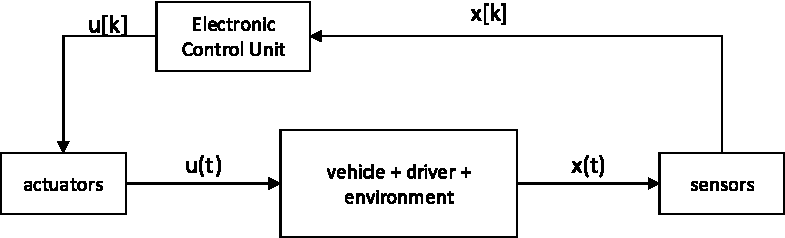
\includegraphics[scale=0.5]{figures/system1_.pdf}
			\caption{The sampled-data control system to be considered.}
			\label{fig:system1}
		\end{center}
	\end{figure}
	
	A test environment can be defined for function verification and validation. The test environment consists a test program in which the function executes its operation, an analysis which checks the function operation and a reporting and logging part. See Figure~\ref{fig:system2}. The test environment may inject artificial errors into the system to verify the function robustness. See Figure~\ref{fig:system3}
	
	\begin{figure}[h]
		\begin{center}
			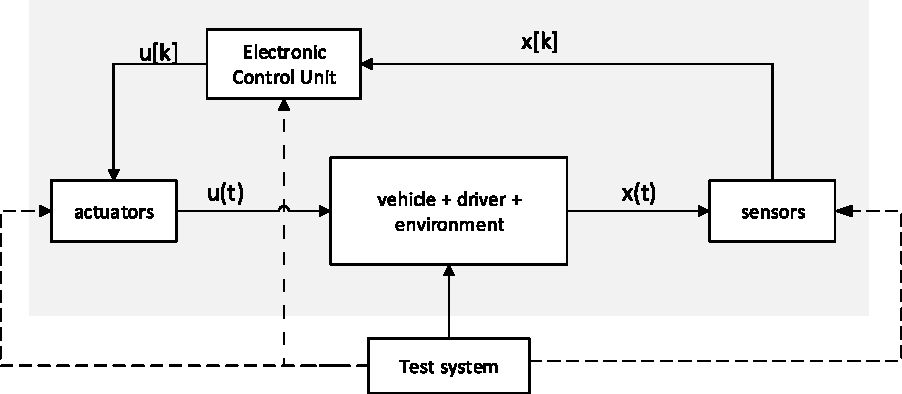
\includegraphics[scale=0.5]{figures/system2_.pdf}
			\caption{The test environment interacts with the vehicle and its driver, defines the simulated environment, the sensors and actuators.}
			\label{fig:system2}
		\end{center}
	\end{figure}
	
	In order to further learn the controller robustness against noise and injected malicious messages into the vehicle communication network an additional test item is proposed over the existing functional verification/validation test setup. The additional test item add randomized sensor signals $a[k]$ into the communication data flow $x[k], k=0, 1, \ldots$ resulting in:.
	
	\begin{equation}
		\begin{aligned}
			z[2l] &= x[k], \\
			z[2l+1] &= a[k], \quad k, l = 0, 1, \dots
		\end{aligned}
	\end{equation}
	
	
	Let $x\in\Rset^n$ be the state variable, $\psi(a, x) = |a-x|$ the noise function and $\psi[k] = |a[k] - x[k]|, k=0,1,\ldots$. The $a[k]$ can be expressed as:
	
	\begin{align}
		a[k] \sim \pi(a[k]|x[k])
	\end{align}
	
	where $\pi(a[k]|x[k])$ is the probability of taking action $a[k]$ in state $x[k]$. See \autoref{fig:system3}.
	
	The noise density can be reduced in a way that not every true sample is followed by a stochastic sensor value.
	
	At each controller action phase $\Delta t$ the ECU decides if it accepts the signal or refuse its use and stay with the previous state. $z[l]$ may present an uneven and timely more frequent sensor value sample series than the regular operation. If the controller accept the sensor value it can be either the true sample $x[k]$ or "close" to the true value i.e. $\psi[k] \in C(x[k-1])$. $C(x[k])$ represent the ECU signal conditioning, safety and security function, it is a set of accepted sensor inputs. If the expected controller behavior $u'(t, \psi)$ is "close" to the undisturbed operation $u(t)$ so its performance $y'(t)$ is also "close" to the specification $y(t)$. 
	
	\begin{align}
		||y'(t) - y(t)|| <= L||u'(t, \psi) - u(t)||
	\end{align}
	
	for some constant $L>0$.
	
	Similarly if the controller rejects sensor value and use only the last accepted sample, its performance shall be acceptable.
	The test system continuously monitors the ECU operation and reports if the added noise brakes or degrades the operation. 
	In order to minimize the execution cost of fuzz testing, the added test component shall minimize the controller output (i.e. degrade its performance), maximize the noise level while keeping the ECU functional $\psi[k] \in C(x[k-1])$.
	
	\begin{align}
		\pi\opt = \min_{\pi}h(x,u')|_{\psi \in C}
	\end{align}
	
	\begin{figure}[h]
		\begin{center}
			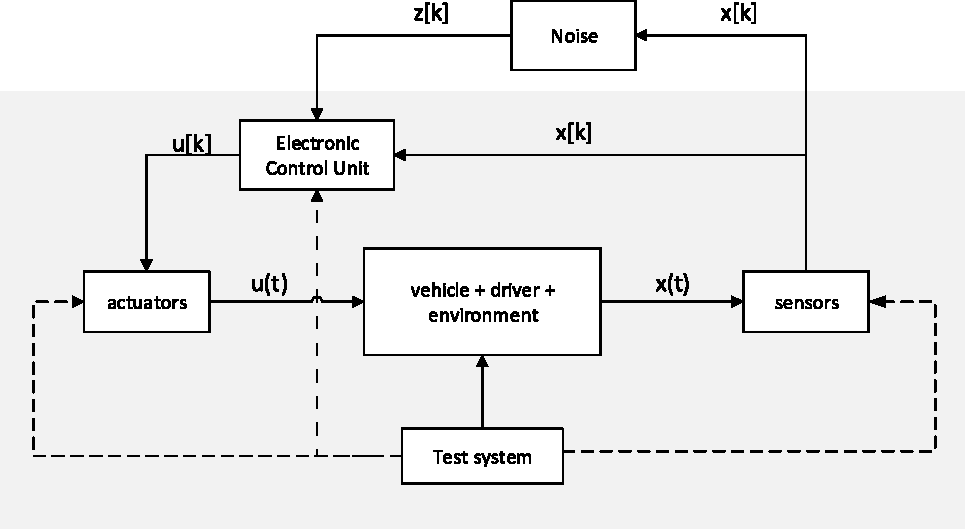
\includegraphics[scale=0.5]{figures/system3_.pdf}
			\caption{The proposed test method consists an additional item which injects noise into the the already existing test architecture.}
			\label{fig:system3}
		\end{center}
	\end{figure}
	
	The additional test item is a Deep Reinforcement Learning actor. The actor gets its observation from the test environment state $x[k]$ and issue its actions as noises $a[k]$.
	The agent contains two components: a policy $\pi$ and a learning algorithm.
	The policy is a mapping from the current environment observation $x[k]$ to a probability distribution of the actions $a$ to be taken. Within an agent, the policy ("test program") is implemented by a function approximator with tunable parameters $\pi_\pparams$ and a specific approximation model, such as a deep neural network.
	The learning algorithm continuously updates the policy learnable parameters based on the actions $a[k]$, observations $x[k]$, and rewards $y[k]$. 
	
	The goal of the learning algorithm is to find an optimal policy $\pi\opt$ that maximizes the expected discounted cumulative long-term reward received during the task \cite{sutton1998reinforcement}.
	
	\subsection{Soft Actor-Critic (SAC) Agent}
	The Soft Actor-Critic (SAC) algorithm is an off-policy reinforcement learning method designed for environments with discrete and continuous action spaces \cite{christodoulou2019soft, haarnoja2018soft}. The action space in the proposed test environment is the injected noise on the sampled signals based on the observation of the true signal values. The actor aims to learn a stochastic policy that maximizes the expected return end entropy. The return in our case is the negative effect on the ECU functional performance. Entropy, in this context, measures the uncertainty or randomness in the policy’s action choices, encouraging the agent to explore more diverse actions rather than settling too quickly on a potentially sub-optimal strategy. By optimizing both reward and entropy, SAC effectively balances exploration and exploitation. The algorithm employs two critic networks to estimate the value of the optimal policy, along with target critics to stabilize learning. It also uses an experience replay buffer to improve sample efficiency.
	
	\begin{figure}[h]
		\begin{center}
			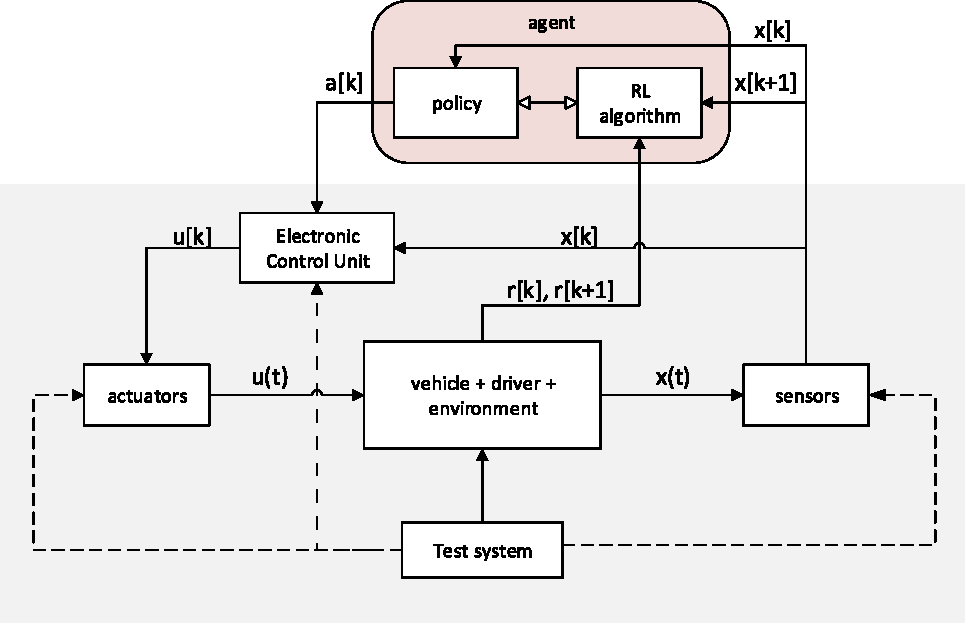
\includegraphics[scale=0.5]{figures/system4.pdf}
			\caption{During learning the RL algorithm continuously update the policy until its performance reaches the desired optimum. When it is used for testing the ECU, the RL algorithm is switched off and the trained policy generates the noise.}
			\label{fig:RL}			
		\end{center}
	\end{figure}
	
	\subsubsection{Maximum Entropy Reinforcement Learning}
	The SAC reinforcement learning problem can be defined as policy search in an a Markov decision process (MDP), defined by a tuple $(\sspace, \aspace, \pdyn, \reward)$. The state space $\sspace$ and action space $\aspace$ are assumed to be continuous, and the state transition probability $\pdyn:\ \sspace \times \sspace \times \aspace \rightarrow [0,\, \infty)$ represents the probability density of the next state $\stp\in\sspace$ given the current state $\st\in\sspace$ and action $\at\in\aspace$. The environment emits a reward $\reward: \sspace \times \aspace \rightarrow  [\rmin,\rmax]$ on each transition. $\rho_\policy(\st)$ and $\rho_\policy(\st,\at)$ are also used to denote the state and state-action marginals of the trajectory distribution induced by a policy $\policy(\at|\st)$.  Besides the standard reinforcement learning objective to learn a policy $\policy(\at|\st)$ to maximize the expected sum of rewards $\sum_t \E{(\st,\at)\sim\rho_\policy}{\reward(\st,\at)}$ the SAC algoritm extends the objective with an entropy term:
	
	\begin{align}
		\label{eq:sql:maxent_objective}
		\policy\opt = \arg\max_{\policy} \sum_{t} \E{(\st, \at) \sim \rho_\policy}{\reward(\st,\at) + \alpha\ent(\policy(\voidarg|\st))}
	\end{align}
	
	The temperature parameter $\alpha$ determines the relative importance of the entropy term against the reward controlling the stochasticity of the optimal policy.
	
	The algorithm uses two parametrized soft Q-functions $\Q_\params(\st, \at)$ as critics and a policy function  $\policy_\pparams(\at|\st)$ as an actor. During training, both the actor and the critics adjust their internal parameters $\pparams$ and $\params$ respectively to improve performance. After training, these parameters are fixed and used by the trained agent. The optimization objective of the actor and critic networks are minimizing the following functions respectively:
	
	\begin{align}
		J_\policy(\pparams) = \E{\st\sim\mathcal{D}}{\E{\at\sim\policy_\pparams}{\alpha \log\left(\policy_\pparams(\at|\st)\right) - Q_\params(\st, \st)}}
	\end{align}
	
	\begin{align}				
		J_\Q(\params) = &\mathbb{E}_{(s_t,a_t)\sim\mathcal{D}} \Bigg[ \frac{1}{2} \Big( \Q_\params(s_t, a_t) - {} \notag \\
		&\Big( \reward(s_t,a_t) + \discount \mathbb{E}_{s_{t+1}\sim\pdyn} \left[ V_{\bar\params}(s_{t+1}) \right] \Big) \Big)^2 \Bigg]							
		\label{eq:q_cost}		
	\end{align}
	
	where $V_{\bar\params}(\stp)$ is the soft state value function:
	
	\begin{align}
		V(\stp) = \E{\at\sim\policy}{\Q_{\bar\params}(\stp, \atp) - \alpha\log\policy_\pparams(\atp|\stp)}
	\end{align}
	
	The discount factor $\discount$ is important for infinite horizon problems to ensure that the sum of expected rewards is finite. To gain further training stability Q-function parameters $\params$ are smoothed with exponentially moving average resulting in $\bar\params$.
		
	\subsection{Use case - ABS braking in a curve}
	
	A modified Matlab/Simulink reference model is utilized for the use case. The vehicle is a 14DOF passenger car with four wheels; the body has six DOFs - longitudinal, lateral, vertical and pitch, yaw and roll, and each wheel has two DOFs — vertical and rolling. The model implements controllers for engine control units (ECUs), transmissions, and antilock braking systems (ABS). The vehicle under control can be described as a continuous-time system. 
	
	\begin{figure}[h]
		\centering
		\includegraphics[width=.6\columnwidth]{figures/actualmodel.jpg}
		\caption{Matlab/simulink model of a vehicle ABS controller test frame with the proposed smart fuzzing test system.}
		\label{FIG:ABS_Simulink}
	\end{figure}
	
		
	The controller (ABS ECU) maximizes the utilization of adhesion in order to efficiently brake the vehicle and keep it on the road i.e. maintain traction and steering control. It operates by rapidly modulating brake pressure through electronic sensors and hydraulic actuators optimizing wheel slips to achieve optimal lateral and longitudinal forces at the wheels, see \autoref{FIG:WheelSlips}. 
	
	The simulation environment contains a five-phase hybrid automaton governing the ABS control logic similar to the one described in \cite{gerard2012improvements}. Each discrete phase of the automaton prescribes specific brake pressure adjustments applied to the caliper, with transitions between phases triggered by slip through wheel speed measurements and vehicle speed estimations. The resulting cyclic behavior induces a repetitive trajectory in the system’s state space.
	
	The simulated ABS ECU is fed with sensor signals sampled from the simulation at every 5 msec and controls the vehicle emergency braking dynamics by actuators with commands at each 5 msec. The sensor signals and actuator commands are converted back and forth to fixed point numbers as they were embedded into CAN frames. The model used has a test "device" which introduces noise into the wheel speed sensor digital data flow: Each captured "true" wheel speed value is followed by a fake wheel speed sample.
		
	\begin{figure}[ht]
		\centering
		\begin{subfigure}[b]{0.48\columnwidth}
			\centering
			\includegraphics[width=\linewidth]{figures/LongitudinalForce_slip.pdf}
		\end{subfigure}
		\begin{subfigure}[b]{0.48\columnwidth}
			\centering
			\includegraphics[width=\linewidth]{figures/LateralForce_slip.pdf}
		\end{subfigure}
		\caption{Wheels are modeled with 2DOF, rotation about spin axis, and vertical displacement. It models the tire using the Magic Formula.\cite{pacejka2005tire}}
		\label{FIG:WheelSlips}
	\end{figure}
			
	In the simulation maneuver the vehicle accelerates up to $16.67\frac{m}{s}$ in a straight line, is keeps constant speed over further $40m$, then suddenly starts an emergency braking and evasive maneuvering. The evasion is realized by a constant turned steering wheel position, which results in turned front axle wheels of $0.42rad$ and $0.56rad$. The whole maneuver is executed on a slippery road with $\mu=0.6$ (this value typically corresponds to a wet asphalt or lightly snow-covered road).
	
	The training uses the same maneuver. Return of an action (noise) is the decreased ability to keep turning while decelerating as much as possible. The episode reward is the sum of the returns during the braking.
		
	\section{Experiments}
	\subsection{Noise injection strategies}	
	
	Conventional fuzzing would inject random noise without being aware of the controller performance. Therefore it can be inefficient if the ECU is equipped with a proper noise filtering algorithm $C(x[k])$. In the experimental plant model a basic filter is implemented in order to simulate realistic controller behavior. If the wheel speed signal is higher than the estimated vehicle speed ($\omega_{w}r_{w} > v_{veh})$) then the signal is dropped or the rear axle wheel speed average is significantly deviates from the input shaft speed of the differential ($|\frac{\omega_{left}+\omega_{right}}{2} - \omega_{is}| < \epsilon$). \autoref{FIG:Performance} shows the importance a proper signal filter, even the above described simple rules can filter out most of the random noise and provide the controller good enough signals to execute a slightly deviating ABS performance.
		
	\begin{figure*}[ht]
		\centering
		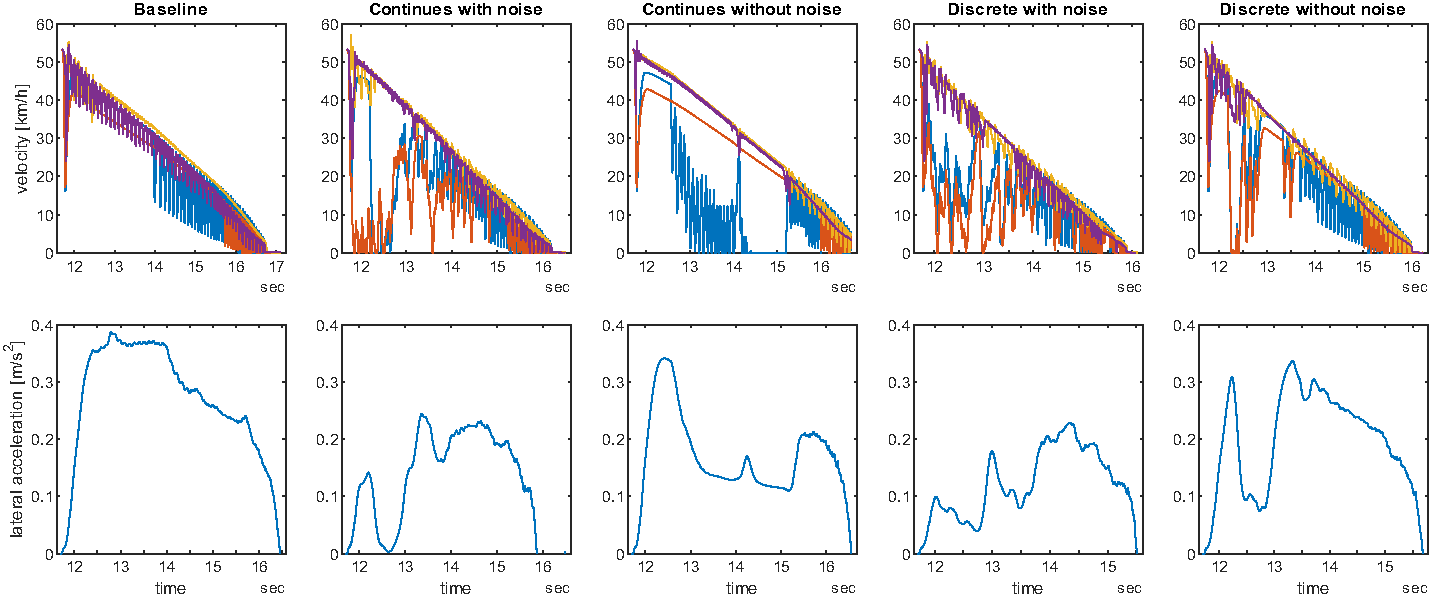
\includegraphics[width=\textwidth]{figures/SAC_all_performance.pdf}
		\caption{Simulation 1: Baseline ABS operation. Simulation 2: a conventional fuzzing of input signals Simulation 3: conventional fuzzing without signal filtering. Simulation 4-7: Fuzzing with a trained agent $Agent_a$ - $Agent_d$.}
		\label{FIG:Performance}
	\end{figure*}		
		
	Four noise injection patterns (i.e. tampering digital wheel speed sensor signals) are tested in the emergency brake use case to achieve optimal test execution parameters. The injected noise is sampled from a Gaussian distribution parameterized with different mean and different distributions.
	
	\begin{enumerate}[a)]
		\item Continuous action space with additional noise.\\
		Let $\mathbf{a}_{min}, \mathbf{a}_{max} \in \mathbf{R}^4$, $\mathbf{a} \in \aspace$ if $\mathbf{a}_{min} \leq \mathbf{a} \leq \mathbf{a}_{max}$ and $a_i \sim \mathcal{N}(\mu_i, \sigma_i^2), i=1,\ldots,4$. The sampled wheel speed sensor signals are mixed with $a_i$ actions resulting in $z_i$ inputs to the ABS controller. $a_1$ is mixed to the front left wheel speed sensor signal, $a_2$ to the front right, and so on. See Figure~\ref{fig:system3}. The action is constant for $\Delta t = 0.1 s$.\\
		\item Continuous action space without additional noise.\\
		The same as above, only the distribution is zeroed $\sigma_i=0, i=1,..4$, resulting in deterministic $\textbf{a}$ noise. The action is constant for $\Delta t = 0.01 s$
		\item Discrete action space with additional noise.\\
		Let $\boldsymbol{\mu} = \{\mu_1,\ldots,\mu_{10} \}$, $\boldsymbol{\sigma} = \{\sigma_1,\ldots,\sigma_{10}\}$ and $\textbf{a} \in \boldsymbol{\mu} \times \boldsymbol{\sigma}$ and $a \sim \mathcal{N}(\mu_i, \sigma_j^2)$ The sampled wheel speed sensor signals are all mixed with the same $a$ action. The action is constant for $\Delta t = 0.1 s$
		\item Discrete action space without additional noise.\\
		The same as above, only the distribution is zeroed again, so $\textbf{a} \in \boldsymbol{\mu}$. The action is constant for $\Delta t = 0.01 s$
	\end{enumerate}                        		
	
	$Agent_a$ is using pattern $a$, $Agent_b$, $Agent_c$ and $Agent_d$ are using patterns $b$, $c$ and $d$ respectively. See \autoref{FIG:TestResults}.
			
	\subsection{Training}
	The trained agent is "disturbing" the ABS operation. ~\autoref{FIG:Performance} shows the baseline operation and the four test cases. The upper graph row shows wheel speeds and at the lower row the lateral acceleration during the braking. The failing ABS control either does not optimally utilize the adhesion resulting in longer stopping distance or in lost control. The test strategy in which real noise is also injected (pattern $a$ and $c$) besides the selected false target signal value shows better results in terms of more degraded overall ABS operation. The $Agent_a$ using continuous action space with noise (pattern $a$) was able to block the front wheels, however the ABS control was able to get back to a better operation range. The best performing agent ($Agent_c$) is the one which utilized a discrete action space efficiently disturbing the performance with frequent over-optimal wheel braking.
	
	\begin{figure*}[hb]
		\centering
		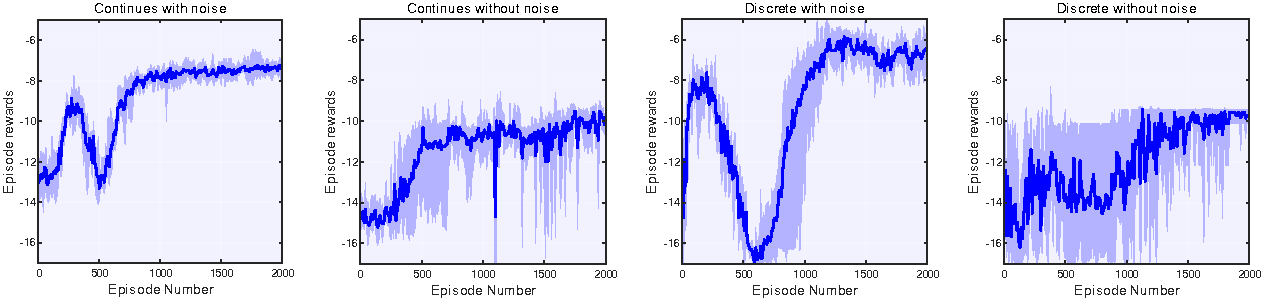
\includegraphics[width=\textwidth]{figures/SAC_all_statistics.pdf}
		\caption{Training curves on continuous control benchmarks. Soft actor-critic (blue and yellow) performs
			consistently across all tasks and outperforming both on-policy and off-policy methods in the most challenging
			tasks.}
		\label{FIG:TrainingResult}
	\end{figure*}		
	
	\begin{figure*}[h]
		\centering
		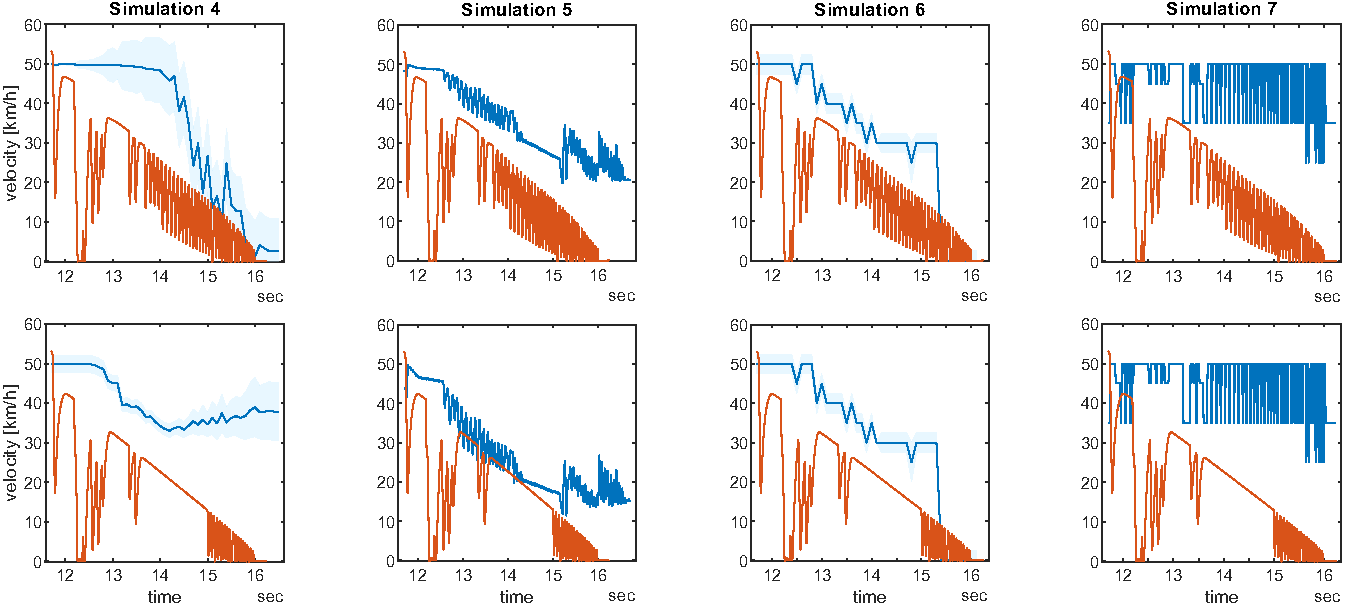
\includegraphics[width=\textwidth]{figures/SAC_all_wheelspeeds.pdf}
		\caption{Result of the optimized test environment. Simulation 4-7: Fuzzing with a trained agents $Agent_a$ - $Agent_d$. The upper row is the speed of the front left wheel and the lower row shows the front right wheel speeds. In each graph wheel speeds are shown in red and the mean value of the noise with blue. The shaded area around the blue curve is the distribution of the random noise.}
		\label{FIG:TestResults}
	\end{figure*}	
	
	Other important factor is the training speed in which the agent in the test arrangement learns their actuation policy. 
	~\autoref{FIG:TrainingResult} shows the ABS braking in a curve (episode) performance degradation (reward). Five different instances of each agent variant with different random seeds were trained, with each performing 2000 episodes. The solid curves corresponds to the mean and the shaded region to the minimum and maximum returns over the five trials.
	Learning of the agent with continuous action space with noise converges its episode award (accumulated lateral acceleration during ABS braking) of $\sim7.5 \frac{m}{s^2}$. These values are achieved from approximately after the 1000th learning iteration. Learning of the agent with continuous action space without noise achieve $\sim10 \frac{m}{s^2}$ a bit earlier, from approximately after the 800th iteration but it struggles to keep it stable. The best performing agent (the one with discrete action space with noise) achieves its stable optimum $\sim6.5 \frac{m}{s^2}$ beyond approximately 1300th iterations. And lastly the worst performing agent reach its peek performance $\sim10 \frac{m}{s^2}$ at the end of the learning schedule at round about 1900-200th iterations.
	
	\begin{table}[hb]		
		\renewcommand{\arraystretch}{1.4} % Increases row spacing
		\centering		
		\vspace{1mm}
		\begin{tabular}{l|c|c|c}			
			\toprule
			Action space & Exp. reward & Max. reward & Speed \\
			\midrule
			Cont. w. noise    & $\sim7.5\frac{m}{s^2}$  & $\sim6.5\frac{m}{s^2}$  & $\sim 1000$                \\
			Cont. wo. noise   & $\sim10\frac{m}{s^2}$   & $\sim8.5\frac{m}{s^2}$ & $\sim 800$                 \\
			Disc. w. noise    & $\sim6.5\frac{m}{s^2}$  & $\sim5\frac{m}{s^2}$   & $\sim 1300$                \\
			Disc. wo. noise   & $\sim10\frac{m}{s^2}$   & $\sim8.3\frac{m}{s^2}$ & $\sim 1900$                \\			
			\bottomrule
		\end{tabular}				
		\caption{Comparison of agents with different action spaces and noise strategies in terms of reward and learning speed.}
		\label{tab:action_space_comparison}
	\end{table}
		
	As shown in \autoref{tab:action_space_comparison} agents with noise in their actions tend to yield the better expected and maximum rewards then those without using noise. The action type whether it is continuous or discrete is more relevant in the learning speed than the presence of noise. 		
	
	\autoref{tab:shared_params} lists the common SAC parameters used in the comparative evaluation in \autoref{FIG:Performance}.
	
	\begin{table}[hb]
		\renewcommand{\arraystretch}{1.1}
		\centering		
		\vspace{1mm}
		\begin{tabular}{l| l }
			\toprule
			Parameter &  Value\\
			\midrule
			optimizer &Adam\\
			actor learning rate & $1 \cdot 10^{-4}$\\
			critic learning rate & $5 \cdot 10^{-4}$\\
			discount ($\discount$) &  0.99\\
			replay buffer size & $10^6$\\
			number of hidden layers (all networks) & 2\\
			number of hidden units per layer & 256\\
			number of samples per minibatch & 64\\
			entropy target & $-\dim\left(\aspace\right)$ \\
			nonlinearity & ReLU\\
			target smoothing coefficient ($\tau$)& 0.001\\
			target update interval & 1\\			
			\bottomrule
		\end{tabular}
		\caption{SAC Hyperparameters}
		\label{tab:shared_params}
	\end{table}
	
	\subsection{Results}
	Using conventional fuzzing the degradation of the lateral acceleration is relatively small, the test does not exploit potential issues of the filter, however the fuzzing has an effect as the simulation without signal filter shows. The accumulated lateral acceleration in the continuous, offset and range action space is 6.47 $\frac{m}{s^2}$, in the continuous and offset only case is 8.57 $\frac{m}{s^2}$, in the discrete, offset and range action space is 4.99 $\frac{m}{s^2}$, in the discrete and offset only case is 8.30 $\frac{m}{s^2}$ 
	The agents with continuous action space has the option to influence ABS control with optimized target deviation signals, while in case of agents with discrete action space the common target deviation is used for both axles. \autoref{FIG:TestResults} shows in the first two columns the different deviation targets and the last two columns the common targets. The resulting wheel speeds are different in the two sides even in the case of common actions due to the turning maneuver. The test trial shows that despite that the agents with side wise separated actions have the option to influence the lateral acceleration with the effect of different side wise braking force, it has not been exploited.
	
	\begin{figure}[h]
		\centering
		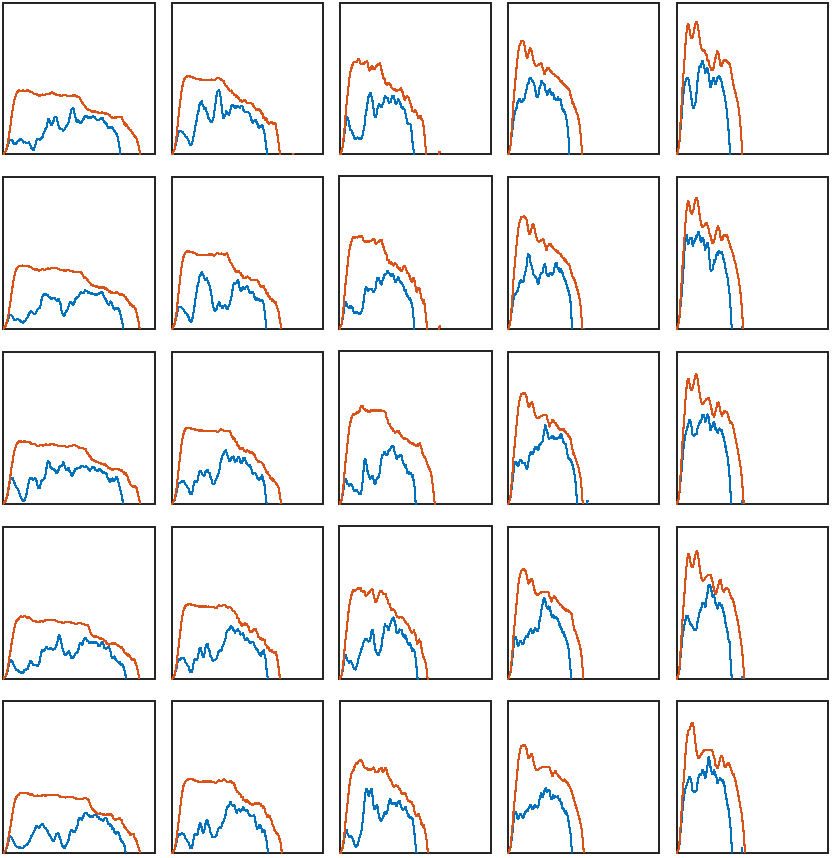
\includegraphics[width=\columnwidth]{figures/AgentPerformanceGrid.pdf}
		\caption{Using the agent of pattern $c$ on different maneuvers. The graphs are showing the lateral acceleration during braking over the braking period. The upper lines in each figure is the base line performance, while the lower line is the result of the trained agent injecting noises.}
		\label{FIG:PerformanceGrid}
	\end{figure}	
	
	The agent is trained on a specific maneuver described earlier, however it still performs on different driving conditions. \autoref{FIG:PerformanceGrid} shows emergency braking on different road surfaces and with different evasions. From left to right the road friction varies as $\mu \in [0.4, 0.5, 0.6, 0.7, 0.8]$ and from top to down as $ valami \in [a b c a]$. As expected the figures show decreasing stopping distances as the road surface becomes drier and wheels have more grip. The agent shows good performance in test cases with low $\mu$ and it is less efficient when the friction is higher. 
	
	The ABS controller has to achieve the goal in which the vehicle stops the quickest but it still can be steered. As \autoref{FIG:WheelSlips} shows if the controller optimizes for a higher slips depending on the road conditions it achieves higher longitudinal braking force, while less lateral force. And vice versa from steering point of view the optimum is at the lower slips. The agents are trained to decrease the ABS performance of steering ability, which resulted in improving the stopping distances. This explains that the graphs show improved stopping distance when agent disturbs the ABS operation. 
			
	\section{Conclusion}
	The proposed test method is verified with simplified model-in-the-loop (MIL) environment with a plant model of a detailed passenger vehicle model. The system under test (SUT) is a simplified Matlab/Simulink ABS controller with a signal conditioning. The ABS receives sensor signal periodically sampled and subsequently converted into a fixed-point representation for further processing.
	The outlined test execution setup showed that the SUT performs significantly worst than the baseline operation. The test environment contains an RL agent which is trained by consecutive execution of the test maneuver. During each maneuver the agent injects noise and evaluate its effect, after the maneuver refines its strategy in order to find the optimal test execution setup.
	The emphasis is on its automatic behavior. It finds the most problematic operation of the system under test without the active guidance of the tester. Mixing noise to the true signal samples will either be filtered out by the signal conditioning infrastructure, used with altered controller performance or in worst case breaks the controller by exploiting a hidden bug. The result of the test shall be evaluated from functional safety point of view: if the agent produce noise within the specification the result shall also be in the acceptable range. However if the agent produced noise is out of specification and the performance is not acceptable, the review signal conditioning performance as well as the assessment of the case from cyber security point of view.
	The proposed setup with the trained agent can be a test bed for the control logic with its signal conditioning infrastructure (model-in-the-loop - MIL), the complete ECU software including all of its functionality (software-in-the-loop - SIL) and finally the real ECU (hardware-in-the-loop). 
	 
	 
	\bibliographystyle{cas-model2-names}	
	\bibliography{References}
				
	
	%\listoftodos		
\end{document}
